%% abtex2-modelo-include-comandos.tex, v-1.9.5 laurocesar
%% Copyright 2012-2015 by abnTeX2 group at http://www.abntex.net.br/ 
%%
%% This work may be distributed and/or modified under the
%% conditions of the LaTeX Project Public License, either version 1.3
%% of this license or (at your option) any later version.
%% The latest version of this license is in
%%   http://www.latex-project.org/lppl.txt
%% and version 1.3 or later is part of all distributions of LaTeX
%% version 2005/12/01 or later.
%%
%% This work has the LPPL maintenance status `maintained'.
%% 
%% The Current Maintainer of this work is the abnTeX2 team, led
%% by Lauro César Araujo. Further information are available on 
%% http://www.abntex.net.br/
%%
%% This work consists of the files abntex2-modelo-include-comandos.tex
%% and abntex2-modelo-img-marca.pdf
%%

% ---
% Este capítulo, utilizado por diferentes exemplos do abnTeX2, ilustra o uso de
% comandos do abnTeX2 e de LaTeX.
% ---
 
\chapter{Background}\label{ch:background}
% ---
\section{Similar Selection Systems}
% ---
\noindent
The system most similar to ours is RIDA$\sp{*}$ (Barley et al., \citeyear{BarleySantiagoOver}). RIDA$\sp{*}$ also selects a subset from a pool of heuristics to guide the A$\sp{*}$ search. In RIDA$\sp{*}$ this is done by starting with an empty subset and trying subsets of size one before trying subsets of size two and so on. RIDA$\sp{*}$ stops after evaluating a fixed number of subsets. While RIDA* is able to evaluate sets of heuristics with only tens of elements. By contrast, the method we propose in this dissertation is able to evaluate sets with thousands of elements.

Rayner et al., (\citeyear{raynersss13}) present an optimization procedure that is similar to ours. In contrast with our work, Rayner et al. limited their experiments to a single objective function that sought to maximize the sum of heuristic values in the state space. Moreover, Rayner et al.'s method performs an uniform sampling of the state space to estimate the sum of heuristic values in the state space. Thus, their method is not directly applicable to domain-independent planning. In this dissertation we adapt Rayner et al.'s approach to domain-independent planning by using Stratified Sampling Chen (\citeyear{chen1992heuristic}) to estimate the sum of heuristic values in the state space. Our empirical results show that \texttt{GHS} minimizing an approximation of A$\sp{*}$'s running time is able to substantially outperform Rayner et al.'s approach in domain-independent planning. 

Our meta-reasoning requires a prediction of the number of nodes expanded by A$\sp{*}$ using any given subset. The prediction system we choose is Stratified Sampling (\texttt{SS} system (Lelis et al., \citeyear{lelis2013predicting})). Even though, \texttt{SS} produce good predictions for Iterative-Deepening A$\sp{*}$, it does not give us good predictions for A$\sp{*}$ because it is unable to detect duplicated nodes during search (Lelis et al., \citeyear{lelis2014estimating}). Although \texttt{SS} does not produce good predictions of the number of nodes generated by A*, we show empirically that SS allows \texttt{GHS} to make good subset selections.

% ---
\section{Problem definition}
% ---

A $SAS\sp{+} planning\ task$ (B$\ddot{a}$ckstr$\ddot{o}$m; Nebel, \citeyear{backstrom1995complexity}) is a 4 tuple $\nabla = \{V, O, I, G\}.$ \textit{V} is a set of \textit{state variables.} Each variable \textit{v} $\in$ \textit{V} is associated with a finite domain of possible $D_{\substack{v}}$. A state is an assignment of a value to every $v \in V.$ The set of possible states, denoted \textit{V}, is therefore $D_{\substack{v_{\substack{1}}}}    \times ... \times D_{\substack{v_{\substack{2}}}}$. \textit{O} is a set of operators, where each operator $o \in O$ is triple $\{pre_{\substack{o}} , post_{\substack{o}}, cost_{\substack{o}}\}$ specifying the preconditions, postconditions (effects), and non-negative cost of \textit{o}. $pre_{\substack{o}}\ and\ post_{\substack{o}}$ are assignments of values to subsets os variables, $V_{\substack{pre_{\substack{o}}}}\ and\ V_{\substack{post_{\substack{o}}}}$, respectively. Operator \textit{o} is applicable to state \textit{s} if \textit{s} and $pre_{\substack{o}}$ agree on the assignment of values to variables in $V_{\substack{pre_{\substack{o}}}}$. The effect of \textit{o}, when applied to \textit{s}, is to set the variables in $V_{\substack{post_{\substack{o}}}}$ to the values specified in $post_{\substack{o}}$ and to set all other variables to the value they have in \textit{s}. \textit{G} is the goal condition, an assignment of values to a subset of variables, $V_{\substack{G}}$. A state is a goal state if it and \textit{G} agree on the assignment of values to the variable in $V_{\substack{G}}$. \textit{I} is the initial state, and the planning task, $\nabla$, is to find an optimal (least-cost) sequence of operators leading from \textit{I} to a goal state. We denote the optimal solution cost of $\nabla$ as $C\sp{*}$. 

% ---
\section{The 8-tile-puzzle case}
% ---
The state space problem illustrated in the Figure \ref{fig:8tilepuzzle_begin} consists in a board with 8 squares named tiles numbered from 1 to 8 and one square without tile and number named empty tile. The goal of the game is to order the tiles in some order. For example: From left to right and up to bottom in the following order 1, 2, 3, 4, 5, 6, 7, 8 and empty tile. This game is called the 8 Sliding-tile puzzle and its objective is to place the tiles in order by moving the numbered tiles into the empty tile. For this case, the goal would be reached by placing the tiles 1, 2 and 3 in the first row, and 4, 5 and 6 in the following row, and 7, 8 and empty tile in the last row.

\iffalse
Schaeffer; Herik, (\citeyear{Schaeffer:2002:GCA:512148.512149}) Any tile horizontally or vertically adjacent to the blank can be slid into that position. The problem is to rearrange the tiles from some random initial configuration into a particular desired goal configuration. The 8-puzzle contains 181,440 reachable states, the 15$-$puzzle contains about $10\sp{13}$ reachable states, and the 24-puzzle contains almost $10\sp{25}$ states.
\fi

\begin{figure}[htb]
\centering
\begin{forest}
 [\usebox\myboxa \hspace*{1.4in} \usebox\myboxb]
 $\node [xshift=-5.5cm,yshift=3.5cm] (A) at (2,0) {Initial};$
 $\node [xshift=1.5cm,yshift=3.5cm] (A) at (2,0) {Goal};$
\end{forest}
\caption{The left tile-puzzle is one possible initial distribution of tiles and the right tile-puzzle is the goal distribution of tiles. Each one represents a state.} \label{fig:8tilepuzzle_begin}
\end{figure}

Instead of using \texttt{DFS} or \texttt{BFS} that will analyze the states encountered, we can obtain heuristics for the 8-sliding-tile puzzle that will help us solve the problem more quickly.

\section{Heuristics}
There exist many state-space algorithms, and one of the most important and well know is A$\sp{*}$ (Hart P. E. et al., \citeyear{hart1968formal}). A$\sp{*}$ uses the $f(s) = g(s) + h(s)$ cost function to guide its search to a solution. $g(s)$ is the cost to go from the start state to state $s$, and $h(s)$ is the estimated cost to go from $s$ to the goal.

\begin{figure}[htb]
\centering
\begin{tikzpicture}
	%\draw[yshift=-1 em, ultra thick] (0,0) [point] -- (5,0) [point] -- (10,0) [point];
	\coordinate (I) at (0,0) (I) node[point=ultra thick, above] {I};
	\coordinate (I1) at (2,0) (I1) node[point=ultra thick, above] {};
	\coordinate (I2) at (4,0) (I2) node[point=ultra thick, above] {};
	\coordinate (I3) at (6,0) (I3) node[point=ultra thick, above] {};
	\coordinate (s) at (8,0) (s) node[point=ultra thick, above] {s};
	\coordinate (I4) at (10,0) (I4) node[point=ultra thick, above] {};
	\coordinate (I5) at (12,0) (I5) node[point=ultra thick, above] {};
	\coordinate (G) at (14,0) (G) node[point=ultra thick, above] {G};
	\draw (I) -- (G);	

\draw [decorate,decoration={brace,amplitude=4pt},xshift=4pt,yshift=14pt]
(8,0) -- (12,0) node [black,midway,yshift=0.5cm] 
{\footnotesize $h(s)=2$};

\draw [decorate,decoration={brace,amplitude=8pt,mirror},xshift=4pt,yshift=-14pt]
(0,0) -- (8,0) node [black,midway,yshift=-0.5cm] 
{\footnotesize $g(s)=4$};


\draw [decorate,decoration={brace,amplitude=6pt,mirror},xshift=4pt,yshift=-14pt]
(8,0) -- (14,0) node [black,midway,yshift=-0.5cm] 
{\footnotesize $h\sp{*}(s)=3$};
\end{tikzpicture}
\caption{Heuristic Search: \textit{I}: Initial state, \textit{s}: Some sate, \textit{G}: Goal state} \label{fig:searchSpace}
\end{figure}

In the Figure \ref{fig:searchSpace} the optimal distance from the initial state $I$ to  the state $s$ is 4 and is represented by $g(s)$. The $h\sp{*}(s) = 3$ represents the optimal distance from $s$ to the goal state $G$, and $h(s) = 2$ is the estimation distance from $s$ to $G$.

A heuristic is admissible if $h(s) \leq h\sp{*}(s)$ for all $s \in V$, where $h\sp{*}(s)$ is the optimal cost of $s$. A heuristic is consistent iff $h(s) \leq c(s,t) + h(t)$ for all states $s$ and $t$, where $c(s,t)$ is the cost of the cheapest path from $s$ to $t$. For example, the heuristic function provided by a pattern database (\texttt{PDB}) heuristic (Culberson and Schaeffer, \citeyear{culberson1998pattern}) is admissible and consistent.

Given a set of admissible and consistent heuristics $\zeta = \{h_{1}, h_{2}, \dots, h_{M}\}$, the heuristic $h_{max}(s,\zeta) = $max$_{h \in \zeta} h(s)$ is also admissible and consistent. When describing our method we assume all heuristics to be consistent. We define $f_{max}(s, \zeta) = g(s) + h_{max}(s, \zeta)$, where $g(s)$ is minimal when A$\sp{*}$ using a consistent heuristic expands $s$. We call an A$\sp{*}$ search tree the tree defined by the states generated by A$\sp{*}$ using a consistent heuristic while solving a problem $\nabla$.

We now show two heuristics for the 8-puzzle.

\subsection{Out of place (O.P)}
This heuristic counts the number of tiles that are out of the goal position. If the tile is not in its goal position, then it counts as one, otherwise it counts as zero. 

\begin{figure}[htb]
\centering
\begin{forest}
 [\usebox\myboxa]
 $\draw[->,xshift=4pt,yshift=14pt] (2,1) -- (4,1);$
 $\node [xshift=1cm,yshift=2cm] (A) at (2,0) {O.P=8};$
 \hspace*{1.8in} 
 %$\rightarrow$  
 [\usebox\myboxb] 
\end{forest}
\caption{Out of place heuristic} \label{fig:8tilepuzzle_oop}
\end{figure}

The tiles numbered with 4, 1, 2, 3, 6, 7, 5, and 8 are out of place, then each tile count as 1 and the sum would be 8, then the heuristic value for this state is 8.

\subsection{Manhatham Distance (M.D)}
This heuristic counts the minimum number of operations that should be applied to any tile to place it in its goal position. Let us explain this with an example: Tile 5 is located on the bottom left of the tile puzzle shown on the left-hand side of Figure \ref{fig:8tilepuzzle_md}, then the minimum number of moves to get tile 5 to its goal position is 2 (either up and right or right and up), both movements equal to 2.

\begin{figure}[htb]
\centering
\begin{forest}
 [\usebox\myboxa]
 $\draw[->,xshift=4pt,yshift=14pt] (2,1) -- (4,1);$
 $\node [xshift=1cm,yshift=2cm] (A) at (2,0) {M.D=1O};$
 \hspace*{1.8in} 
 %$\rightarrow$  
 [\usebox\myboxb] 
\end{forest}
\caption{Manhatham distance heuristic} \label{fig:8tilepuzzle_md}
\end{figure}

Tile 4 requires one move to get to its goal position;
Tile 1 requires one;
Tile 2 requires one;
Tile 3 requires one;
Tile 6 requires one;
Tile 7 requires one;
Tile 5 requires two moves;
Tile 8 requires two;
The sum of required moves is 10.

Out-of-place and Manhattan distance are heuristics that use domain knowledge. There are methods that create heuristics without using domain knowledge. Barley et al., (\citeyear{BarleySantiagoOver}) call them heuristic generators.

\section{Heuristic Generators}
Some heuristic generators work by creating abstractions of the original problem space. \texttt{PDBs} (Culberson and Schaeffer, \citeyear{culberson1998pattern}) are an effective way of generating heuristics, \texttt{PDBs} work as follows: The search space of the problem is abstracted into a smaller state space that can be enumerated with exhaustive search. The distance of all abstracted states to the abstracted goal state are stored in a lookup table, which can be used as a heuristic function for the original state space.

\section{Using a Set of Heuristics}
One well-know approach to take advantage of heuristics is to compute the maximum of all heuristics $\zeta$. For example, given two heuristics h1 and h2, the maximum of h1 and h2 will tend to yield a more informed heuristic than h1 and h2 individually.

The heuristic generators can create hundreds or even thousands of heuristics and we need to figure it out how to take advantage of this large set of heuristics. In fact, there exist different ways to take advantage of those heuristics, however we need to take into account that if we want to use all the heuristics created by the heuristic generator, the resulting heuristic would be too expensive to guide search. This is because, the main problem involved would be the time required to evaluate all the heuristics for each node in the search tree.

\section{Heuristic Subset}
Let's suppose we have to run our meta-reasoning considering that we have a fixed amount of memory $M$. Then, one question is raised: How many heuristics our system should consider? Holte et al., (\citeyear{holte2006maximizing}) observed that maximizing over $N$ pattern databases of size $M/N$, for $N < M$, can produce a search tree size smaller than the search tree size generated by using a single pattern database of size $M$. Thus we will use heuristic generators to create a large number of heuristics to fill the amount M of memory available.

Heuristic generator systems can create a large number of heuristics. Let us suppose $|\zeta| = $ 1000 heuristics were created and that our meta-reasoning for example selects $N =$ 50 heuristics. This would imply count the following number of combinations one can get from solving the combinatorial problem: $${1000\choose 50} \approx 10\sp{85} possibilities$$

\iffalse
\section{Problem Domains}
Some of the problems we are trying to solve are the optimal domains for International Planning Competition (\texttt{IPC}).

\subsection{Blocks world}
The domain is not an optimal domain, but we include it in this part because we consider that is a domain that must be explained in order to understand other more complex. This domain consists on a set of blocks on the table and a hand robot. The blocks might be distributed over another block or over the table. The goal is to find the plan where the robot places the blocks from one distribution of blocks to another.

\begin{figure}[htb]
\centering
\begin{forest}
[\usebox\myboxblockteststar \hspace*{0.2in} \usebox\myboxblockgreenone \hspace*{1.5in} \usebox\myboxblocktestend]
\end{forest}
\caption{Blocks world with three blocks.}\label{fig:probblocks}
\end{figure}

The solution shown in Figure \ref{fig:probblocks} would be the following plan: unblock number 3 from block number 2; stack block number 2 on block number 1; and finally, stack block number 3 on block number 2.

%\iffalse
\subsection{Barman}
This domain consists in a set of drinks that would be available to one robot barman create different combination of drinks. The goal is to find the plan of the robot's actions.
%This domain consists in a set of drink dispensers, glasses and a shaker that are used by a robot barman to create combination of drinks. The objective is to find the plan of the robot's actions that create the drinks.
%\fi

\subsection{Floortile}
This domain consists in a robot that paints patterns in floor tiles using one color at a time, but changing the spray guns to any available. The objective is to find the plan to paint floor tiles only in front. This domain still have problems painting behind since the search reaches to dead-end.

\subsection{Nomystery}
This domain consists in a truck that transport and load/unload packages from one node to another considering the resources consumption. For example, the fuel is measured based on the weighted graph and each move consumes the edge weight in fuel. The goal is to find the plan that transport the packages based on the resource constrained.

\subsection{Openstacks}
This domain consists in a manufacture that produce only one product at a time. This is because we want to avoid production stop when changing from one product to another. The time that last to produce all the elements from one product is called ``open'' and the time each element of that product to be stored during the production is called ``stack''. This is an optimization problem that require to order the products to be made in order to maximize the number of stacks that are in simultaneously.

Finding a plan for this problem could be make it using a domain-specific algorithm, however finding an optimal solution is hard.

\subsection{Parking}
This domain develops a system to park a set of cars from one set to another. Double-parked are allowed, but not triple-parked.

\subsection{Sokoban}
This domain consists in a agent and a set of blocks. The agent has to push the blocks in a specified goal location. 

\begin{figure}[!htb]
\begin{center}
  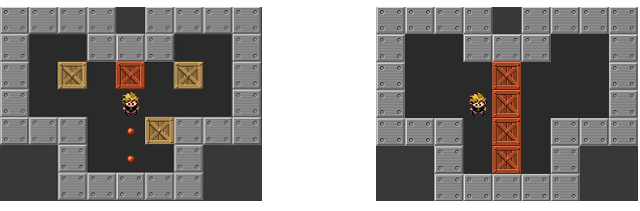
\includegraphics[width=12cm,scale=0.5]{images/sokoban_star_end}
\end{center}
\caption{Sokoban with four blocks solved. (Aymeric du Peloux, \citeyear{sokoban2010})}\label{fig:img_sokoban_solved}
\end{figure}

The solution shown in Figure \ref{fig:img_sokoban_solved} is to use the agent to push blocks located in the left figure to the goal distribution of blocks in the right figure.
\fi

\bigskip

In the next Chapter, we will introduce the meta-reasoning proposed for selecting heuristics.

\clearpage